\section{A hybrid transaction implementation}\label{sec:hybrid}

\begin{figure}[t]\begin{center}%
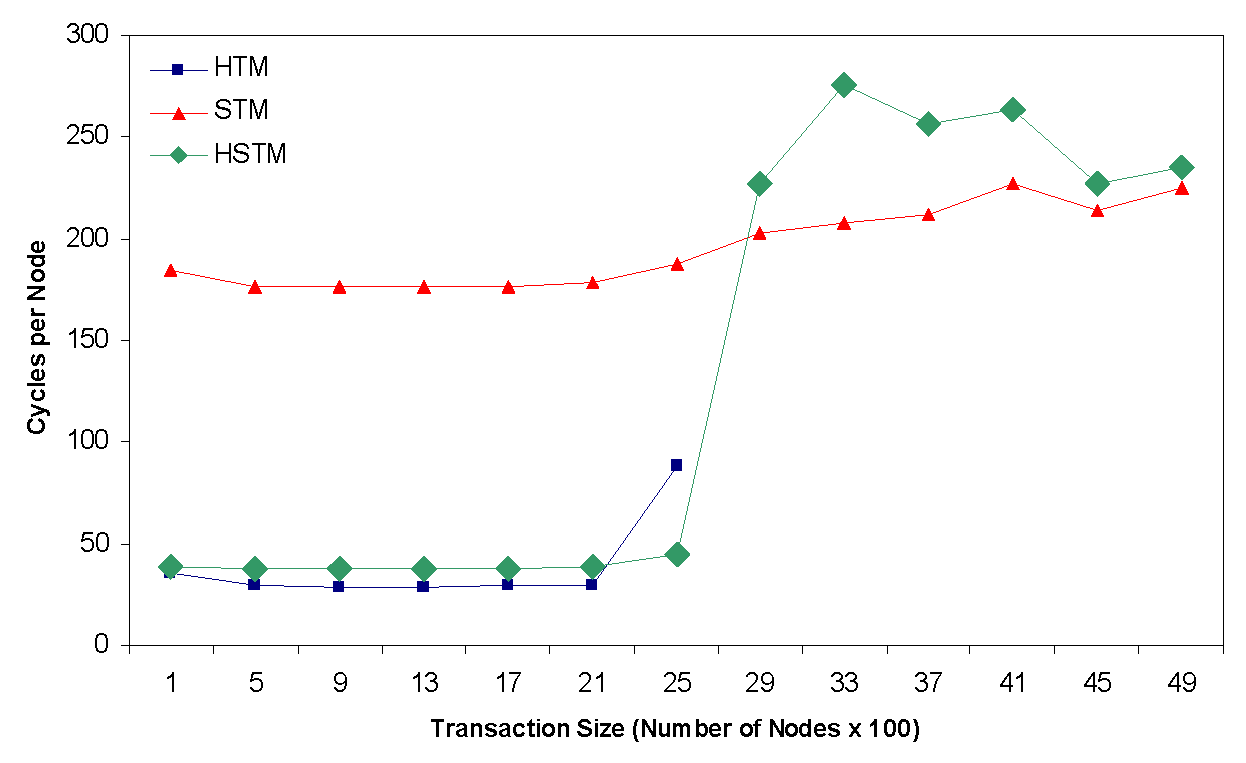
\includegraphics[width=3.25in,clip=true]{Figures/sean_lie_6b}%
\end{center}%
\caption[Hybrid performance on simple queue benchmark.]
{Performance (in cycles per node push on a simple queue
  benchmark) of LTM~\cite{AnanianAsKuLeLi04} (HTM), the
  object-based system presented in this paper (STM) and a hybrid
  scheme (HSTM).}%
\label{fig:hybrid}%
\end{figure}
It is worth considering if a low-level HTM can yield benefits other
than efficient implementations of large-object operations.  In fact,
\figref{hybrid} presents research showing that we can combine the
strengths of our object-based software transaction system with a
fast bounded-size HTM.  In the figure, combining the systems is done
in the most simple-minded way: all transactions are begun in
LTM~\cite{AnanianAsKuLeLi04},
and after any abort the transaction is restarted in the
object-based software system.
  The field flag mechanism described in
\secref{flagfield} ensures that software transactions properly abort
conflicting hardware transactions --- when the software scribbles
\FLAG over the original field the hardware will detect the conflict.
Hardware transactions must perform
the \texttt{ReadNT} and \texttt{WriteNT} algorithms to ensure they
interact properly with concurrent software transactions, although these
checks can be done in software (they do not need to be part of the
hardware HTM mechanism).  In the figure, the read barriers were done
in software, and caused a 2.2x slowdown for the (very small) hardware
transactions.  This is a pessimistic figure: no special effort was
made to tune code or otherwise minimize slowdown, and the processor
simulated had limited ability to exploit ILP (2 ALUs and 4-instruction
issue width).  Even so, the read barriers might be a worthwhile target
for hardware support \cite{ClickTeWo05}.

As a fortuitous synergy, hardware support for small transactions may
also be used to implement the software transaction implementation's
Load Linked/Store Conditional sequences, which may not
otherwise be available on a target processor.
